\documentclass[12pt]{article}
\usepackage[margin=1in]{geometry}
\usepackage{amsmath,amsthm,amssymb,amsfonts}
\usepackage{float}
\usepackage{color}
\usepackage{xcolor}
\usepackage{graphicx}
\usepackage[utf8]{inputenc}
\usepackage{biblatex}
\usepackage{tikz}
\usepackage[tok, page]{appendix}
\usepackage{listings}

% tikz style stuff
\usetikzlibrary{arrows}
\tikzstyle{block} = [rectangle, draw, fill=orangeCoral, text width = 1.5em, text centered, minimum height = 2em]
\tikzstyle{blockTurf} = [rectangle, draw, fill=turfGreen!50, text width = 1.5em, text centered, minimum height = 2em]
\tikzstyle{blockAlgae} = [rectangle, draw, fill=algaeRed!45, text width = 1.5em, text centered, minimum height = 2em]
\tikzstyle{blockParrot} = [rectangle, draw, fill=parrotBlue!50, text width = 1.5em, text centered, minimum height = 2em]
\tikzstyle{line} = [thick, ->, >= stealth]
\tikzstyle{noblock} = [rectangle, draw = none]

\definecolor{orangeCoral}{HTML}{FFC996}
\definecolor{turfGreen}{HTML}{BDD2B6}
\definecolor{algaeRed}{HTML}{CF0000}
\definecolor{parrotBlue}{HTML}{A7D0CD}

\addbibresource{main.bib}

\title{Effects of Overfishing on Coral Reef Ecosystems\\Coral Reefsearchers}
\author{Aaron Bumagat, Michelle Luces, Henry Song\\University of Guam}
\date{\today}

\begin{document}
\maketitle
% tulai
\section{Introduction}
Coral reefs play a crucial role in the marine's ecosystem as it serves a purpose for an abundance of marine life. Additionally, healthy coral reefs benefit the economy as it provides jobs and businesses through tourism. Unfortunately, in the recent years the health of coral reefs have been declining due to several factors. According to a 2008 world coral reef status report, it predicts that 15\% of all coral are in danger of disappearing within 10-20 years, and 20\% within 20-40 years \textsuperscript{\cite{05_quintero_machuca_cotto_bradley_ríos-soto_2016}}. 

With climate change rates increasing, one of the prevalent factors affecting coral reefs is rising sea temperatures, which leads to mass bleaching of corals. Other destructive environmental factors include ocean acidification, nutrient flow from run-off \textsuperscript{\cite{05_quintero_machuca_cotto_bradley_ríos-soto_2016}}. Another factor that contributes to the decline of healthy coral reefs are due to human activities, such as exploitative fishing practices or pollution \textsuperscript{\cite{04_mathanalysis}}. 

Because a handful of coral species are considered to be threatened, efforts in measuring the resiliency factors of a coral reef has been of interest to many. In one study, ecological factors were studied and scored in which resistance, recovery, and resilience were taken into account. It claimed the top three ecological factors that contribute a coral's resiliency is its species type, temperature variability, and nutrients for pollution run-off \textsuperscript{\cite{02_Riegl_Purkis_Model}}. 

The objective of this paper is to analyze how Guam's reef ecosystem will change over the coming decades, focusing on the impact of overfishing of parrotfish. By setting up a compartment model and subsequent system of differential equations, we are able to model the dynamics of the ecosystem in response to different parameter and compartment values. This will allow us to analyze and predict the effect of overfishing on Guam's coral reef ecosystem. In addition, our analysis will include the application of education game theory in order to quantify the human factor in overfishing.

% objectives of research question, brief explanation of math model
%\section{Objectives}


\section{Modeling}
\subsection{Coral Reef Ecosystem Model}
\begin{center}
    \begin{tikzpicture}{node distance = 1cm, auto}
        \node(leftofC) [noblock] {}; 
        \node(C) [block, right of = leftofC, node distance = 1.5 cm] {C};
        \node(P) [blockParrot, right of = C, node distance = 4 cm] {P};
        \node(belowofC) [noblock, below of = C, node distance = 3 cm]{};
        \node(M) [blockAlgae, right of = belowofC, node distance = 3 cm] {M};
        \node(T) [blockTurf, left of = belowofC, node distance = 3 cm] {T};
        \node(rightofP) [noblock, right of = P, node distance = 1.5 cm]{};
        \node(aboveofP) [noblock, above of = P, node distance = 1.5 cm]{};
        \node(aboveofC) [noblock, above of = C, node distance = 1.5 cm]{};
        \node(belowofP) [noblock, below of = P, node distance = 1.5 cm]{};
        \node(aboveofT) [noblock, above of = T, node distance = 0.08 cm]{};
        \node(diagonalofT) [noblock, right of = aboveofT, node distance = 3 cm]{};
        \draw[dashed, ->] (P) --node[above]{} (diagonalofT);
        \draw[line] (P) --node[above]{$\sigma$} (C);
        \draw[line] (C) --node[left]{$a$} (M);
        \draw[line] (P) --node[above]{$h$} (rightofP);
        \draw[line] (P) --node[left]{$\mu_{2}$} (aboveofP);
        %\draw[line] (C) --node[left]{$d$} (aboveofC);
        \draw[line] (belowofP) --node[right]{$q$} (P);
        \begin{scope}[transform canvas = {xshift = -.15cm}]
            \draw[line](T) -- node[left]{$r$} (C);
        \end{scope}
        \begin{scope}[transform canvas = {xshift = .15cm}]
            \draw[line](C) --node[right]{$\mu_{1}$} (T);     
        \end{scope}
        \begin{scope}[transform canvas = {yshift = .1cm}]
            \draw[line] (M) --node[above]{$g$} (T);
        \end{scope}
        \begin{scope}[transform canvas = {yshift = -.15cm}]
            \draw[line] (T) --node[below]{$\gamma$} (M);
        \end{scope}
        \caption{Flowchart of coral reef ecosystem}
    \end{tikzpicture}
\end{center}

% assumptions and description of model
We assume that the (i) system is closed, (ii) time dimensions are measured over one years, and (iii) macroalgae is the only predator for coral. Corals are assumed to (iv) recruit and overgrow algal turfs and that they are overgrown by macroalgae \textsuperscript{\cite{04_mathanalysis}}. Macroalgae are also assumed (v)colonize dead coral by spreading vegetative over algal turfs \textsuperscript{\cite{04_mathanalysis}}. In addition, (vi) the natural death rate of coral is nonexistent and (vii) algal turfs and macroalgae do not have a death rate (see Fig. 1).

%Represented above is our general compartment model. While this version is a rough draft, it represents the compartments that we wish to include in our model. Included in our model is our $S$ compartment, which represents all susceptible corals, our $E$ compartment representing all exposed corals, our $I$ compartment representing our infected corals, and our $R$ compartment representing recovered corals. While this follows the standard SEIR model layout, we included an $H$ compartment to account for human factors. This is in order to assess how the human factor may directly or indirectly affect the typical "life" cycle of corals. \par
%The $H$ compartment allows to factor in the human factor to the overall equation, however in order to achieve this, we must implement education game theory. This is in order to model human factors such as education about corals, ignorance, and various other factors. By using education game theory, we are able to visualize which strategy is dominant between humans and corals, and reflect this strategy in our overall compartment model.

\subsection{Differential Equations}
C, T, and M are proportions of coral, algal turf, and macroalgae cover on the ocean floor, respectively,  where $C+M+T=1$ to signify the proportion of each population is a selected area. P is the population of the parrotfish that inhabit the coral reef ecosystem in proportion to the maximum carrying capacity. The coral reef dynamics are described as a system of nonlinear differential equations \textsuperscript{\cite{13_blackwood_hastings_mumby_2010}}: 
\begin{align}
    \begin{split}
        \frac{dC}{dt} &= rTC + \sigma P C- (aM+\mu_{1})C\\
        \frac{dP}{dt} &= qP \left( 1-\frac{P}{\beta C} \right) - P \left( h+\mu_{2} \right)\\
        \frac{dT}{dt} &= \mu_{1}C + \frac{g(P)M}{M+T} - T(rC+\gamma M)\\
        \frac{dM}{dt} &= (aC+ \gamma T)M - \frac{g(P)M}{M+T}
    \end{split}
\end{align}

where: 
\begin{align*}
&g(P) = \frac{\alpha P}{\beta}, \\
and\\
&\frac{g(P)M}{M + T} \text{ is the proportion of grazing that affects macroalgae} \textsuperscript{\cite{13_blackwood_hastings_mumby_2010}}.
\end{align*}

%See Table 1 for 



\subsection{Parameter Values}
\begin{table}[H]
    \centering
    \begin{tabular}{c p{9cm} c c}
        \hline
        Parameter & Description & Rate & Units\textsuperscript{\cite{12_noaa_report}\cite{04_mathanalysis}\cite{13_blackwood_hastings_mumby_2010}}\\
        \hline
        \hline
        $\mu_{1}$ & natural death rate of coral reefs & 0.15\textsuperscript{\cite{16_wolanski_richmond_mccook_2004}} & $\frac{1}{year}$\\ %12
        $\mu_{2}$ & natural death rate of parrotfish & 0.22\textsuperscript{\cite{12_noaa_report}} & $\frac{1}{year}$\\ %8
        $a$ & rate that coral is overgrown by macroalgae & 0.1\textsuperscript{\cite{11_zikkah_anggriani_supriatna_2020}} & $\frac{1}{year}$\\ %13
        $r$ & rate that coral recruit to overgrow algal turfs & 10\textsuperscript{\cite{16_wolanski_richmond_mccook_2004}} & $\frac{1}{year}$\\ %12
        %$g$ & grazing rate that parrotfish graze macroalgae without distinction from algae turfs & $\frac{kg}{yrs}$\\
        $\gamma$ & rate that macroalgae spread vegetative over algal turfs & 0.8\textsuperscript{\cite{11_zikkah_anggriani_supriatna_2020}} & $\frac{1}{year}$\\ %13
        $q$ & intrinsic growth rate for parrotfish & 0.47\textsuperscript{\cite{12_noaa_report}} & $\frac{1}{year}$\\ %8
        $\beta$ & carrying capacity of parrotfish & 21* & n/a\\
        $h$ & harvesting rate for parrotfish & 0.14\textsuperscript{\cite{12_noaa_report}} & $\frac{1}{year}$\\ %8
        $\alpha$ & maximum grazing intensity & 1* & n/a\\
        $\sigma$ & rate that parrot fish bite coral & 0.01*& $\frac{bites}{year}$\\
        \hline
    \end{tabular}
    \caption{Model Parameters}
    \label{tab:my_label}
\end{table}
\textit{* = estimated values}

% graphs
\subsection{Graphs}
Using MatLab (See Appendix \ref{appendix:A}), we were able to model the dynamics using our preliminary rates. This was achieved by changing the C, M, \& T proportions. Below are the graphs that were were able to achieve:\\
\begin{figure}[H]
    \centering
    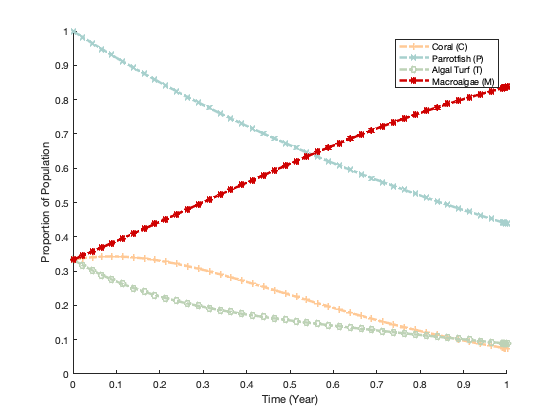
\includegraphics[width=0.7\textwidth]{Latex/Figures/initial_matlab_plot.png}
    \caption{Initial Conditions: $C = T = M = \frac{1}{3}$, and $P = 1$}
    \label{fig:initial_plot}
\end{figure}
\begin{figure}[H]
    \centering
    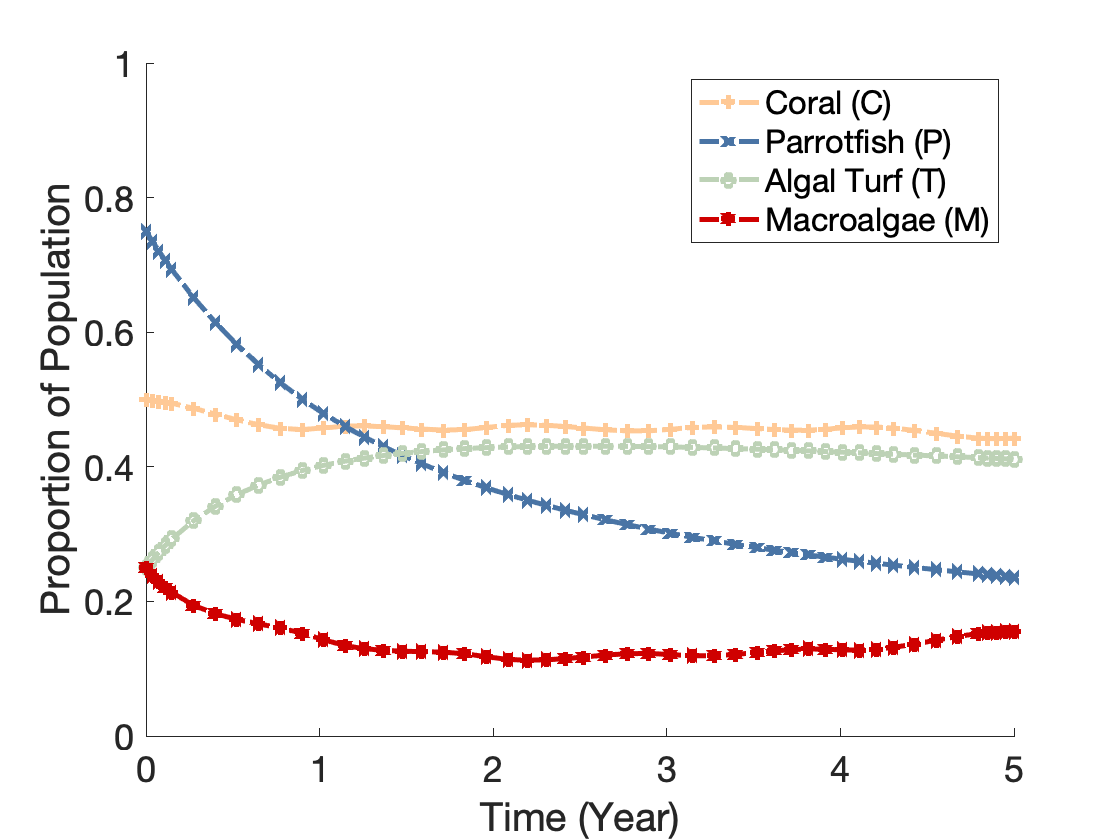
\includegraphics[width=0.7\textwidth]{Latex/Figures/0.5C_0.25T_0.25M.png}
    \caption{Initial Conditions: $C = \frac{1}{2}$, $T = M = \frac{1}{4}$, and $P = 1$}
    \label{fig:coral_dominant}
\end{figure}
\begin{figure}[H]
    \centering
    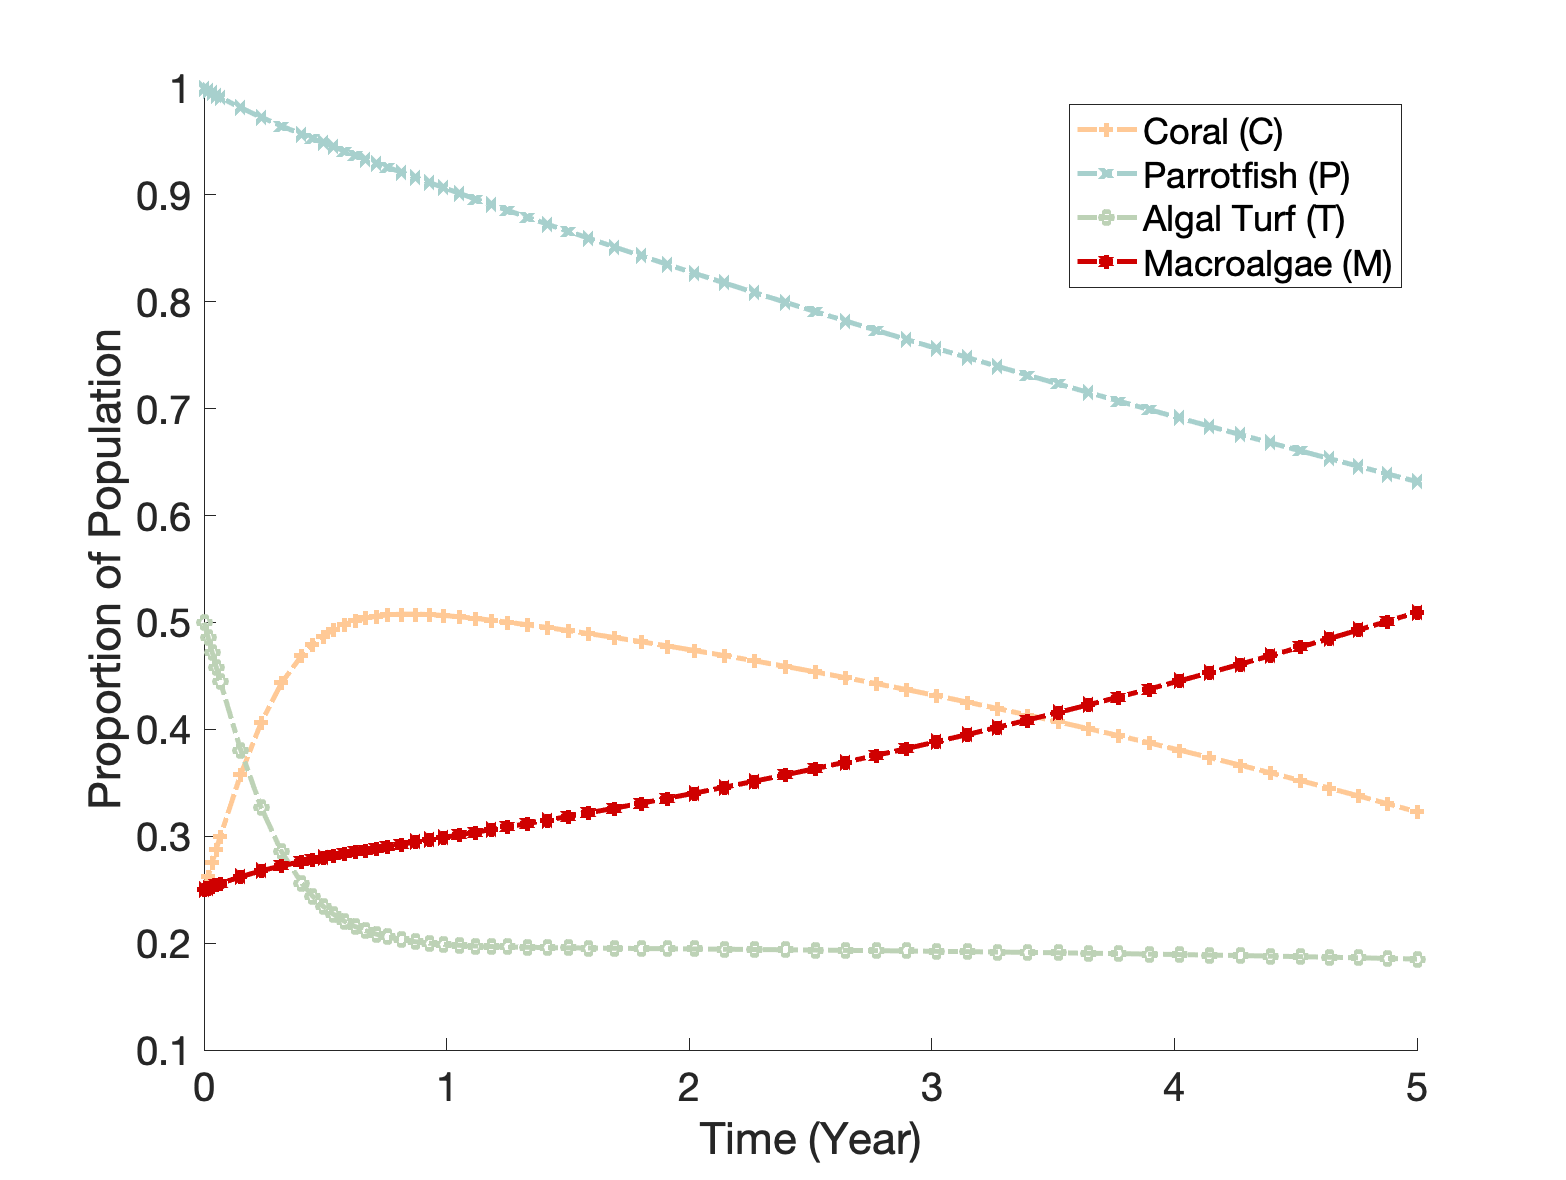
\includegraphics[width=0.7\textwidth]{Latex/Figures/0.25C_0.5T_0.25M.png}
    \caption{Initial Conditions: $T = \frac{1}{2}$, $C = M = \frac{1}{4}$, and $P = 1$}
    \label{fig:turf_dominant}
\end{figure}
\begin{figure}[H]
    \centering
    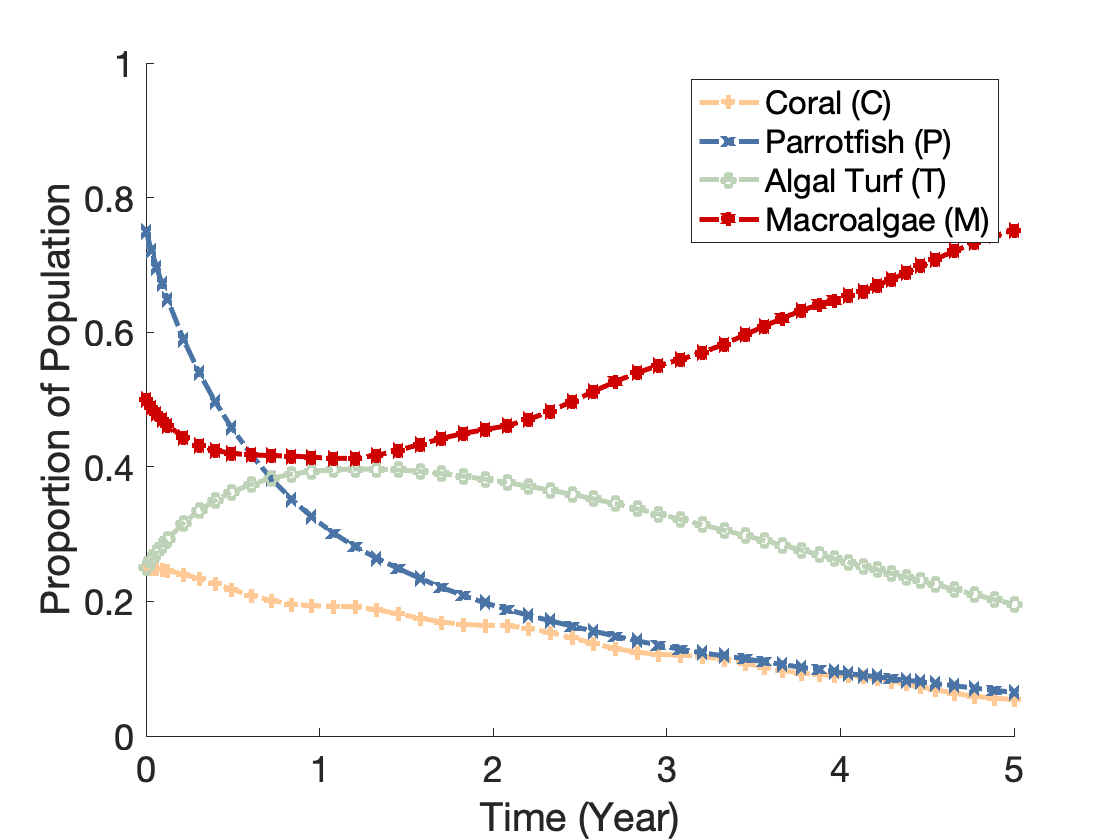
\includegraphics[width=0.7\textwidth]{Latex/Figures/0.25C_0.25T_0.5M.png}
    \caption{Initial Conditions: $M = \frac{1}{2}$, $C = T = \frac{1}{4}$, and $P = 1$}
    \label{fig:macroalgae_dominant}
\end{figure}\\
As we can see in Figures \ref{fig:initial_plot}, \ref{fig:coral_dominant}, \ref{fig:turf_dominant}, \& \ref{fig:macroalgae_dominant}, as the parrot fish population decreases, the macroalgae proportion increases. In addition, as the macroalgae proportion increases, the coral proportion decreases, and subsequently the algal turf proportion decreases as well.\\

%\subsection{Education Game Theory}

\section{Literature Review}
Throughout this week, our group has dedicated a large portion of time to reviewing scholarly articles and research publications relevant to our areas of research. This aspect of performing our research is crucial as, through literature review, we are able to gather information, techniques, methods, data, results, and many other variables that we are able to use in our own research. \par
Our faculty mentors have graciously provided several research publications related to the overall study coral reef ecosystems in order to stimulate creativity in creating our own research topic. These papers are as follow:
\begin{itemize}
    \item Assessing relative resilience potential of coral reefs to inform management\textsuperscript{\cite{01_assesing_relative}}
    \item Model of coral population response to accelerated bleaching and mass mortality in a changing climate\textsuperscript{\cite{02_Riegl_Purkis_Model}}
    \item Prioritizing Key Resilience Indicators to Support Coral Reef Management in a Changing Climate\textsuperscript{\cite{03_prioritize}}
    \item Mathematical analysis of coral reef models\textsuperscript{\cite{04_mathanalysis}}
    \item A Mathematical Model of Coral Reef Response to Destructive Fishing Practices with Predator-Prey Interactions\textsuperscript{\cite{05_quintero_machuca_cotto_bradley_ríos-soto_2016}}
    \item From bee species aggregation to models of disease avoidance: The Ben-Hur effect\textsuperscript{\cite{06_yong_herrera_castillo-chavez_2016}}
    \item Vaccination and the theory of games\textsuperscript{\cite{07_bauch_earn_2004}}
    \item The effect of fishing on hysteresis in Caribbean coral reefs \textsuperscript{\cite{13_blackwood_hastings_mumby_2010}}
\end{itemize}
These articles provide valuable insight in various areas of coral reef research from parameters and conditions to modeling and application. In particular, each of these papers gave us insight on how other researchers approached their problems, how they created and modified their methods, and how they produced results based on their models and equations. 

\section{Acknowledgements}
Support for the Young Scholars Research Experience in Mathematics (YSREM)  is through the MAA Tensor SUMMA Program. Support for the MAA National Research Experience for Undergraduates Program (NREUP) is provided by the National Science Foundation (Grant Number DMS-1950644). Support for the NSF EPSCoR project, Guam Ecosystems Collaboratorium for Corals and Oceans (GECCO) is provided by the National Science Foundation (Grant Number DMS-1946352).
Special thanks to Dr. Bastian Bentlage, our faculty mentors (Dr. JaeYong Choi, Dr. HyunJu Oh, \& Dr. Leslie Aquino), and our Research Assistants (Jaron Bautista \& Regina-Mae Dominguez).

\newpage
\appendix
    \section{MatLab Code}
        \label{appendix:A}
        Below is the MatLab code used to calculate and verify the process of calculating $\mathscr{R}_{0}$:
        \begin{center}
            \lstinputlisting[language=Matlab]{./Source Code/Compartment_Model_DiffEq.m}
        \end{center}
        
\newpage
% \bibliography{main}
% \bibliographystyle{plain}
\printbibliography

\end{document}